\newpage
\noindent When you click the \textbf{Green Flag}, the stage looks like this:
\begin{center}
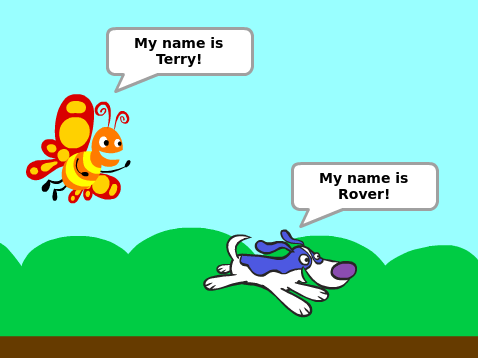
\includegraphics[scale=.5]{q4_stage.png}
\end{center}

\noindent 4a. \textbf{Circle} the script that ran for the butterfly. \\ \\
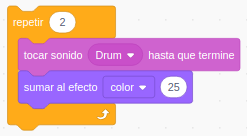
\includegraphics[scale=.3,valign=t]{q4_script0.png} \hspace{1cm}
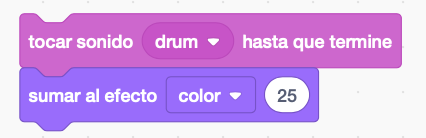
\includegraphics[scale=.3,valign=t]{q4_script1.png} \hspace{1cm}

\includegraphics[scale=.3,valign=t]{q4_script2.png} \hspace{1cm}

\includegraphics[scale=.3,valign=t]{q4_script3.png} \hspace{1cm}
\vspace{1cm}


\noindent 4b. \textbf{Circle} the script that ran for the dog. \\ \\
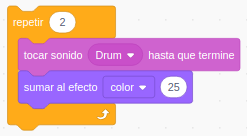
\includegraphics[scale=.3,valign=t]{q4_script0.png} \hspace{1cm}
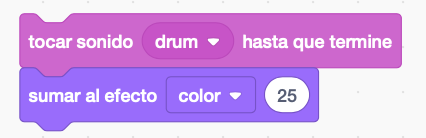
\includegraphics[scale=.3,valign=t]{q4_script1.png} \hspace{1cm}

\includegraphics[scale=.3,valign=t]{q4_script2.png} \hspace{1cm}

\includegraphics[scale=.3,valign=t]{q4_script3.png} \hspace{1cm}
\vspace{1cm}

\noindent \dotfill

\noindent Compare the two scripts below:
\begin{center}
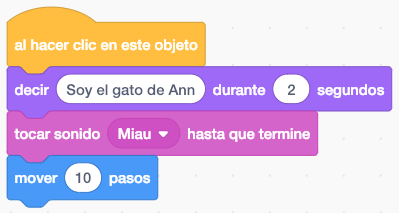
\includegraphics[scale=.3,valign=t]{q5_script0.png} \hspace{0.5in}

\includegraphics[scale=.3,valign=t]{q5_script1.png}
\end{center}

\noindent 5. \textbf{Circle} what is true:
\renewcommand{\theenumi}{\Alph{enumi}}
\begin{enumerate}
\item They do different actions. 
\item They do the same actions in a different order.
\item There is no difference.
\end{enumerate}
\noindent \dotfill \\

\newpage